\chapter{Methodology and Design}

\section{Design Process}\label{sec:overview}

The study follows the design process shown in Figure \ref{fig:method3}: experiments that measure how a deployed fraud model behaves under drift and label delay, a framework designed around their results, and an evaluation of that framework on three datasets.

\begin{figure}[htbp]
  \centering
  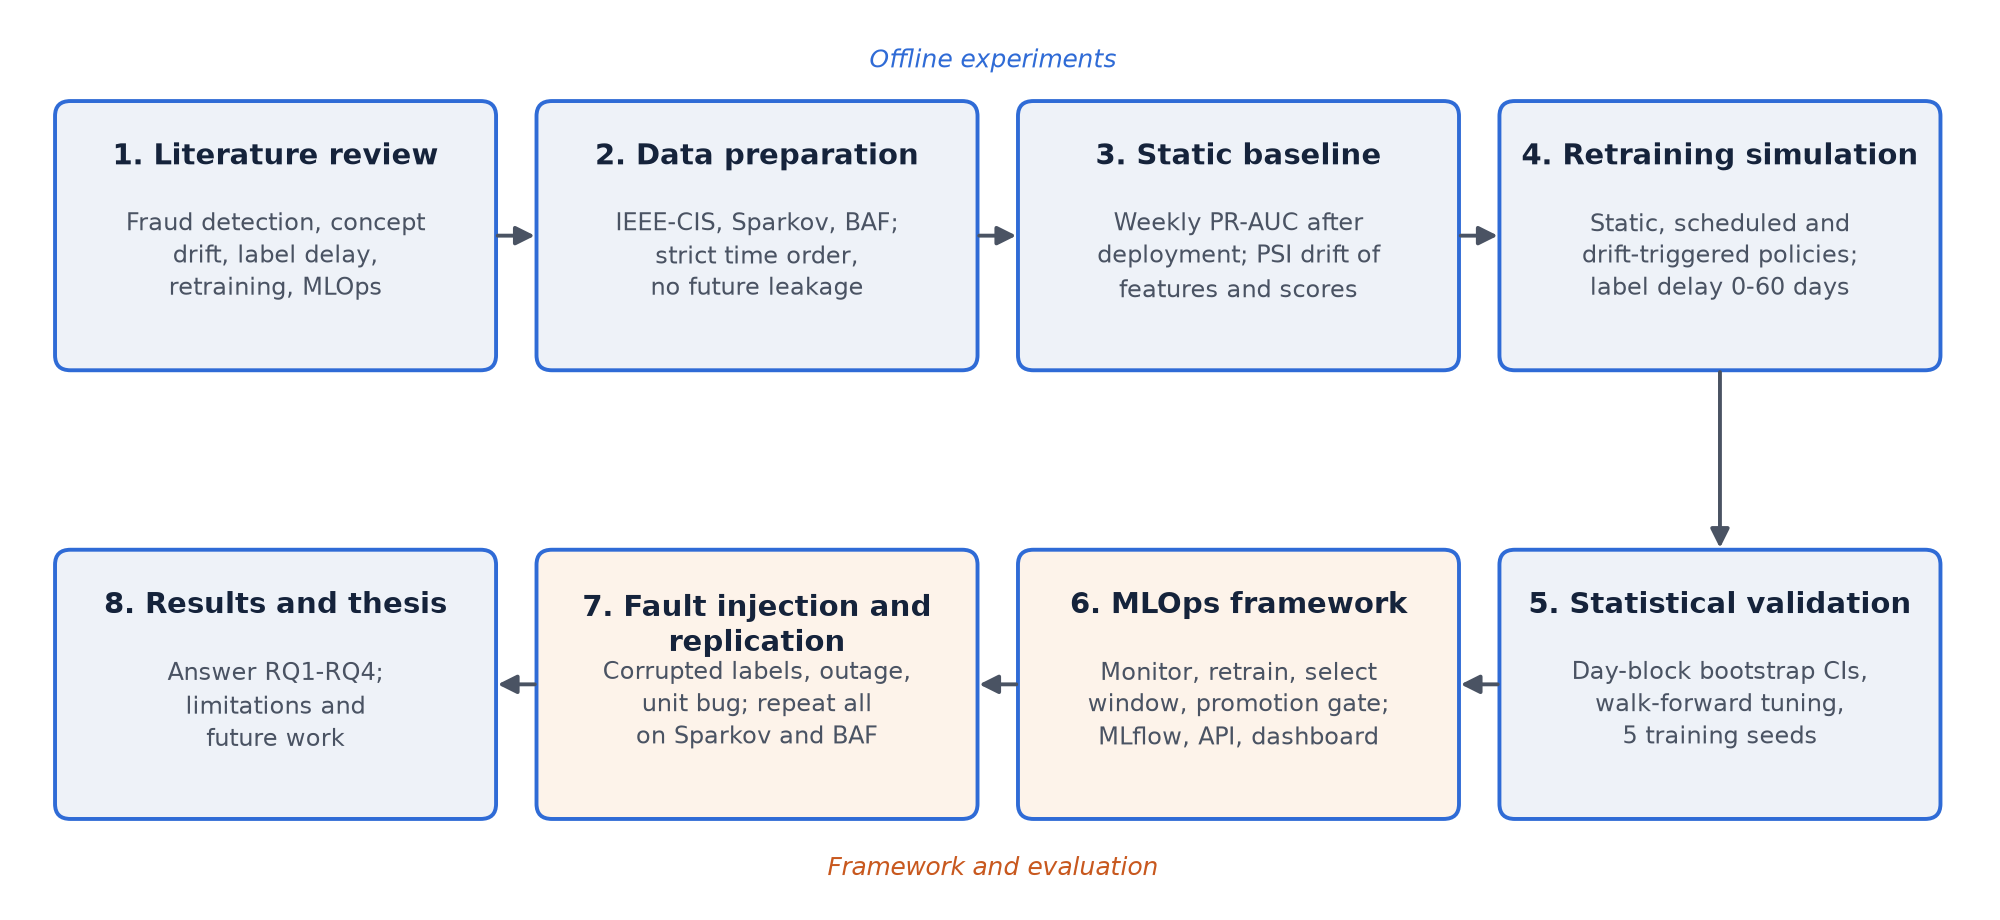
\includegraphics[width=\textwidth]{figures/methodology_3ds.png}
  \caption{Methodology overview: the experiments on three datasets, the framework and its evaluation}
  \label{fig:method3}
\end{figure}

\subsection{Research Design}\label{sec:design}

This study is an empirical, simulation-based investigation followed by the design and evaluation of a software framework. Chapter 2 showed that the claims made for drift-triggered retraining rest mostly on artificial drift, single datasets and labels that arrive immediately \cite{shakil2025,wong2025,yelleti2025}. We therefore first measure, on public fraud data with natural drift, how a deployed model behaves and which retraining policy works best under label delay (research questions RQ1 to RQ3), and only then design the framework around the result and test it (RQ4). The study follows the workflow in Figure \ref{fig:method}.

Three principles guide every experiment. First, \textbf{time is respected}: a model is only trained on transactions that happened, and whose labels were available, before the period it is evaluated on \cite{menezes2025}. Second, \textbf{the deployment is simulated, not imagined}: each dataset is replayed as a stream, week by week, and the label delay is applied explicitly, as described by Dal Pozzolo et al. \cite{dalpozzolo2018}. Third, \textbf{differences must survive uncertainty}: every comparison is reported with a confidence interval, the settings of competing strategies are tuned with the same procedure, and the key results are repeated with several training seeds and on a second dataset.

The rest of this section describes the simulated deployment under label delay (Section \ref{sec:deploy}), the retraining strategies (Section \ref{sec:strategies}), the drift and performance measures (Section \ref{sec:measures}), the statistical validation (Section \ref{sec:validation}) and the evaluation of the framework, including fault injection (Section \ref{sec:faults}). Section \ref{sec:spec} specifies the model and the framework, Sections \ref{sec:collection} and \ref{sec:data} describe the data, Section \ref{sec:plan} the project plan, and Section \ref{sec:impl} the implementation.

\subsection{Simulated Deployment under Label Delay}\label{sec:deploy}

The stream is replayed in steps of seven days, from the stream start to the end of the data. At each step, three things happen in order: the strategy checks which labels are available and decides whether to retrain; if it retrains, a new model is trained and immediately replaces the old one; and the current model scores the transactions of the next seven days. The scores of each week are kept, together with the version of the model that produced them. In production the transactions would arrive through a streaming platform such as Kafka or Flink, as in the real-time pipelines of Kaushik et al. \cite{kaushik2025}; replaying recorded data instead makes every experiment exactly repeatable.

Label delay is modelled as a fixed number of days \textit{d} between a transaction and the moment its label can be used. At time \textit{t}, the labelled data available for monitoring and training is

\begin{equation}
  \mathcal{L}(t) = \{\, x_j : t_j \le t - d \,\}
  \label{eq:labelled}
\end{equation}

where \textit{t\textsubscript{j}} is the time of transaction \textit{x\textsubscript{j}}. The first model is trained at the stream start under the same rule, so it never sees labels it could not have had. We evaluate delays of 0, 15, 30 and 60 days. A delay of 0 corresponds to the assumption made by most retraining studies \cite{yelleti2025,wong2025}; 30 to 60 days corresponds to the time a cardholder typically needs to notice a fraudulent charge and file a dispute \cite{dalpozzolo2018}. Investigator feedback on a few alerted transactions, which arrives faster in a real system \cite{dalpozzolo2018}, is not modelled: every label arrives after the same delay. This makes the setting slightly pessimistic for performance-based triggers, a point we return to in the discussion.

\subsection{Retraining Strategies}\label{sec:strategies}

Five strategies are compared, covering the options described in Section 2.1 \cite{pulicharla2019,dalpozzolo2018}. They are summarised in Table \ref{tab:strategies}.

{\footnotesize
\begin{longtable}{>{\raggedright\arraybackslash}p{0.19\textwidth}>{\raggedright\arraybackslash}p{0.28\textwidth}>{\raggedright\arraybackslash}p{0.23\textwidth}>{\raggedright\arraybackslash}p{0.23\textwidth}}
\caption{Retraining strategies compared in the simulation (default settings)}\label{tab:strategies}\\
\toprule
\textbf{Strategy} & \textbf{When it retrains} & \textbf{Training data} & \textbf{Needs labels to decide?} \\
\midrule
\endfirsthead
\toprule
\textbf{Strategy} & \textbf{When it retrains} & \textbf{Training data} & \textbf{Needs labels to decide?} \\
\midrule
\endhead
Static & Never & History before the stream & - \\ \midrule
Periodic expanding & Every 14 days & All labelled data so far & No \\ \midrule
Periodic sliding & Every 14 days & Labelled data of the last 60 days & No \\ \midrule
Drift: score PSI & PSI of the model's scores over the last week, against its validation scores, exceeds 0.1 (at least 14 days apart) & All labelled data so far & No \\ \midrule
Drift: performance & PR-AUC on newly matured labels falls more than 15\% below the reference (Equation \ref{eq:perftrigger}; at least 14 days apart) & All labelled data so far (or the last 60 days in tuned variants) & Yes (delayed) \\ \bottomrule
\end{longtable}
}

The \textbf{static} model is the reference: it is trained once at the stream start and never updated. The two \textbf{periodic} strategies retrain on a fixed schedule and differ only in their training data: the expanding window uses all labelled data so far, while the sliding window keeps only the most recent 60 days and forgets older patterns.

The \textbf{score-PSI} strategy is a typical label-free drift trigger \cite{shakil2025,wong2025}. It compares the distribution of the scores the model produced over the last week with the scores it produced on its own validation data, using the PSI defined in Section \ref{sec:measures}, and retrains when the PSI exceeds 0.1, the usual boundary between a stable and a shifted population. It can react immediately because it needs no labels.

The \textbf{performance} strategy is an error-based trigger in the spirit of DDM and ADWIN \cite{yelleti2025,aldaoud2025}, adapted to delayed labels. At each step it computes the model's PR-AUC on transactions whose labels matured during the last 14 days and that the model was not trained on, provided they contain at least 30 frauds. It retrains when

\begin{equation}
  \mathrm{AP}_{\mathrm{live}}(t) < (1 - \tau)\, \mathrm{AP}_{\mathrm{ref}}
  \label{eq:perftrigger}
\end{equation}

where AP\textsubscript{live}(\textit{t}) is that live PR-AUC, $\tau$ is the tolerance (0.15 by default), and AP\textsubscript{ref} is either the model's validation PR-AUC or its first live measurement. Both drift strategies wait at least 14 days between retrains, so that one drift episode does not trigger a series of retrains.

Each strategy is run at each label delay, with exactly the same data, model settings and random seed, so that the only difference between runs is the retraining decision and the training window. Models trained on identical windows are cached and reused across strategies, which makes the large number of runs feasible and guarantees that identical decisions give identical models.

\subsection{Drift and Performance Measures}\label{sec:measures}

\textbf{Population Stability Index.} Drift in a feature or in the model's scores is measured with the PSI, which compares a current distribution with a reference distribution \cite{wong2025}:

\begin{equation}
  \mathrm{PSI} = \sum_{i=1}^{B} (c_i - r_i)\,\ln\frac{c_i}{r_i}
  \label{eq:psi}
\end{equation}

where the reference values are divided into \textit{B} = 10 bins at their deciles, \textit{r\textsubscript{i}} and \textit{c\textsubscript{i}} are the shares of reference and current values in bin \textit{i}, missing values form a bin of their own, and shares are floored at 10\textsuperscript{-6} to avoid division by zero. A PSI below 0.1 is usually read as stable, 0.1 to 0.25 as a moderate shift and above 0.25 as a major shift. For the baseline analysis, the PSI is computed for the ten most important features of the static model (by total gain) and for its scores, in every time bin against the training period.

\textbf{PR-AUC.} Fraud is rare and investigators can only review the highest-scored alerts, so the main measure is the area under the precision-recall curve, computed as average precision \cite{dalpozzolo2018}:

\begin{equation}
  \mathrm{AP} = \sum_{n} (R_n - R_{n-1})\,P_n
  \label{eq:ap}
\end{equation}

where \textit{P\textsubscript{n}} and \textit{R\textsubscript{n}} are the precision and recall at the \textit{n}-th threshold of the ranked scores. Unlike accuracy, PR-AUC is not inflated by the large number of legitimate transactions, and unlike ROC-AUC it focuses on how clean the top of the alert list is \cite{abdelnaby2023}. A model with no skill has a PR-AUC equal to the fraud rate.

\textbf{Mean weekly PR-AUC.} In the stream, different weeks are scored by different model versions, whose scores are not calibrated to each other. Computing a single PR-AUC over all weeks would mix these scales and penalise strategies that retrain often, even when every one of their models ranks transactions well. We therefore compute PR-AUC separately for each week \textit{w} of the stream and report the mean over the \textit{W} weeks:

\begin{equation}
  \overline{\mathrm{AP}} = \frac{1}{W} \sum_{w=1}^{W} \mathrm{AP}_w
  \label{eq:weekly}
\end{equation}

Weeks without any fraud are skipped. The lowest weekly PR-AUC, the number of retrains and the F1-score at each model's own threshold are reported as secondary measures.

\subsection{Statistical Validation}\label{sec:validation}

\textbf{Paired day-block bootstrap.} Weekly PR-AUC is noisy, especially when a week contains only a few hundred frauds, and consecutive transactions are correlated. Confidence intervals are therefore computed with a bootstrap that resamples whole days rather than single transactions. Within every week, the days of that week are drawn with replacement, and the mean weekly PR-AUC is recomputed. The same resampled days are used for every strategy, so differences between strategies are paired and much of the shared noise cancels out. We use 500 resamples and report 95\% percentile intervals. A difference is considered reliable when its interval excludes zero.

\textbf{Walk-forward tuning.} A fair comparison requires that every strategy has good settings, chosen without looking at the data it is evaluated on. All 190 configurations in Table \ref{tab:grid} are run over a tuning stream that starts at 35\% of the rows, earlier than the evaluated stream. The evaluated stream is divided into folds of four weeks. At the start of each fold, each family (static, schedule, drift performance) selects the configuration with the highest score

\begin{equation}
  J(c) = \overline{\mathrm{AP}}(c) - \kappa \cdot \frac{N_{\mathrm{retrain}}(c)}{\text{number of 4-week periods}}
  \label{eq:objective}
\end{equation}

computed only on weeks whose labels have matured by the start of the fold, that is, on information that would really have been available. $\kappa$ = 0.002 is a small cost per retrain that breaks ties in favour of simpler configurations. The selected configuration's results on the fold are then recorded, and the next fold repeats the selection. The result is an honest estimate of how each family would perform if an operator tuned it with the information available at the time.

{\footnotesize
\begin{longtable}{>{\raggedright\arraybackslash}p{0.23\textwidth}>{\raggedright\arraybackslash}p{0.47\textwidth}>{\raggedright\arraybackslash}p{0.24\textwidth}}
\caption{Settings searched by walk-forward tuning (190 configurations)}\label{tab:grid}\\
\toprule
\textbf{Family} & \textbf{Settings searched} & \textbf{Configurations} \\
\midrule
\endfirsthead
\toprule
\textbf{Family} & \textbf{Settings searched} & \textbf{Configurations} \\
\midrule
\endhead
Static & - & 1 \\ \midrule
Schedule & Expanding window, period 7, 14 or 28 days; sliding window, period 7, 14 or 28 days and window 30 or 60 days & 9 \\ \midrule
Drift: performance & Tolerance 0.05, 0.1, 0.15, 0.2 or 0.3; monitoring window 7, 14 or 28 days; minimum gap 7, 14 or 28 days; reference = validation PR-AUC or first live measurement; training data = all or last 60 days & 180 \\ \bottomrule
\end{longtable}
}

\textbf{Training seeds.} The bootstrap only covers the randomness of the evaluation sample. LightGBM also has randomness in training, through row and feature subsampling. The key configurations are therefore re-run with five random seeds (42, 1, 2, 3 and 4) at label delays of 0 and 30 days, and for each comparison we report the mean and spread of the difference and the number of seeds in which its sign holds.

\textbf{Replication.} Finally, the whole sequence, from the static baseline through the delay sweep, walk-forward tuning, seeds and the framework replay, is repeated unchanged on Sparkov and BAF, with the same scripts and settings. A finding that holds on IEEE-CIS but not on the other datasets is reported as dataset-specific.

\subsection{Framework Evaluation and Fault Injection}\label{sec:faults}

The framework is evaluated by running it over the evaluated stream of each dataset as if it were live, with a label delay of 30 days. The replay uses the same data store, MLflow registry and model code as a deployment would. Its mean weekly PR-AUC is compared with the offline simulation of the same policy, which checks that the framework reproduces the experimental results, and with the static model. To evaluate window selection, four versions of the framework are replayed on each dataset on the same machine: a static model, a 60-day window, all history, and automatic selection. The four replays share one cache of trained models, so a model with the same training data is trained only once and the versions differ only in their decisions.

A retraining pipeline that runs automatically will eventually train on bad data. To test whether the framework's safeguards stop such models, we inject the faults in Table \ref{tab:faults} into selected retraining jobs of the replay (by default the second and fourth scheduled retrains). The faults imitate common pipeline failures: a misaligned join, an outage of the chargeback feed, and a unit change between training and serving. In the first three, only the data read by the training job is corrupted, while the production feature path and the label store stay correct. The fourth corrupts the label store itself, which the gate also reads, and represents a failure the gate cannot see by design; it tests whether the safety net limits the damage.

{\footnotesize
\begin{longtable}{>{\raggedright\arraybackslash}p{0.23\textwidth}>{\raggedright\arraybackslash}p{0.38\textwidth}>{\raggedright\arraybackslash}p{0.33\textwidth}}
\caption{Faults injected into retraining jobs to test the safeguards}\label{tab:faults}\\
\toprule
\textbf{Fault} & \textbf{What goes wrong} & \textbf{Real-world cause} \\
\midrule
\endfirsthead
\toprule
\textbf{Fault} & \textbf{What goes wrong} & \textbf{Real-world cause} \\
\midrule
\endhead
Label shuffle & Labels are permuted within the training window, so they no longer match their transactions & A misaligned join in the training job \\ \midrule
Label loss & 80\% of frauds in the training window are recorded as legitimate & An outage of the chargeback feed \\ \midrule
Feature unit bug & The five most important numeric features of the live model are multiplied by 100 in training only & A unit change (e.g. cents and dollars) between training and serving \\ \midrule
Upstream label shuffle & The label store itself is corrupted, so the promotion gate also reads wrong labels & Corruption at the source; a known blind spot \\ \bottomrule
\end{longtable}
}

Each fault scenario is replayed twice, once with the promotion gate and once without it, and compared with a clean replay. A safeguard is considered effective if the run with the fault and the safeguard stays close to the clean run, while the run without the safeguard loses performance. Each scenario uses its own MLflow store, so the main registry is never affected.

\section{Design (Model) Specification}\label{sec:spec}

This section specifies the fraud detection model used throughout the study and the components of the drift-aware continuous learning framework.

\subsection{Fraud Detection Model}\label{sec:model}

All experiments use LightGBM, a gradient boosted decision tree library, with the settings in Table \ref{tab:hyper}. Gradient boosted trees are strong and widely used models for tabular fraud data \cite{uddin2026,amekoe2024}, they handle missing values and categorical features natively, and they train fast enough to be retrained hundreds of times. Amekoe et al. also found that batch-trained boosted trees remain competitive with incremental learners when labels arrive late \cite{amekoe2024}, which is exactly the setting of this study. The goal is not to find the best possible classifier, as many static studies do \cite{mienye2023,abdelnaby2023,sohony2018}, but to keep one strong and realistic model fixed so that differences between retraining strategies can be attributed to the strategies alone. No resampling such as SMOTE is used, because it can distort the evaluation \cite{dang2021}; class imbalance is handled by weighting the fraud class instead, a cost-sensitive approach that Somasundaram and Reddy also used to handle imbalance in a drifting fraud stream \cite{somasundaram2019}.

Figure \ref{fig:modelarch} shows the architecture of the model. Each transaction is described by its features, 431 on IEEE-CIS, 16 on Sparkov and 29 on BAF. LightGBM builds an ensemble of decision trees one after another, each with up to 256 leaves, and every new tree is fitted to the errors that the trees before it still make. Training stops when the validation AUC has not improved for 100 rounds, at most after 2,000 trees. For a new transaction, the outputs of all trees are summed into a score \textit{F}(\textit{x}), which a sigmoid function turns into a fraud probability between 0 and 1; the transaction is flagged as fraud when this probability reaches the decision threshold described below.

\begin{figure}[htbp]
  \centering
  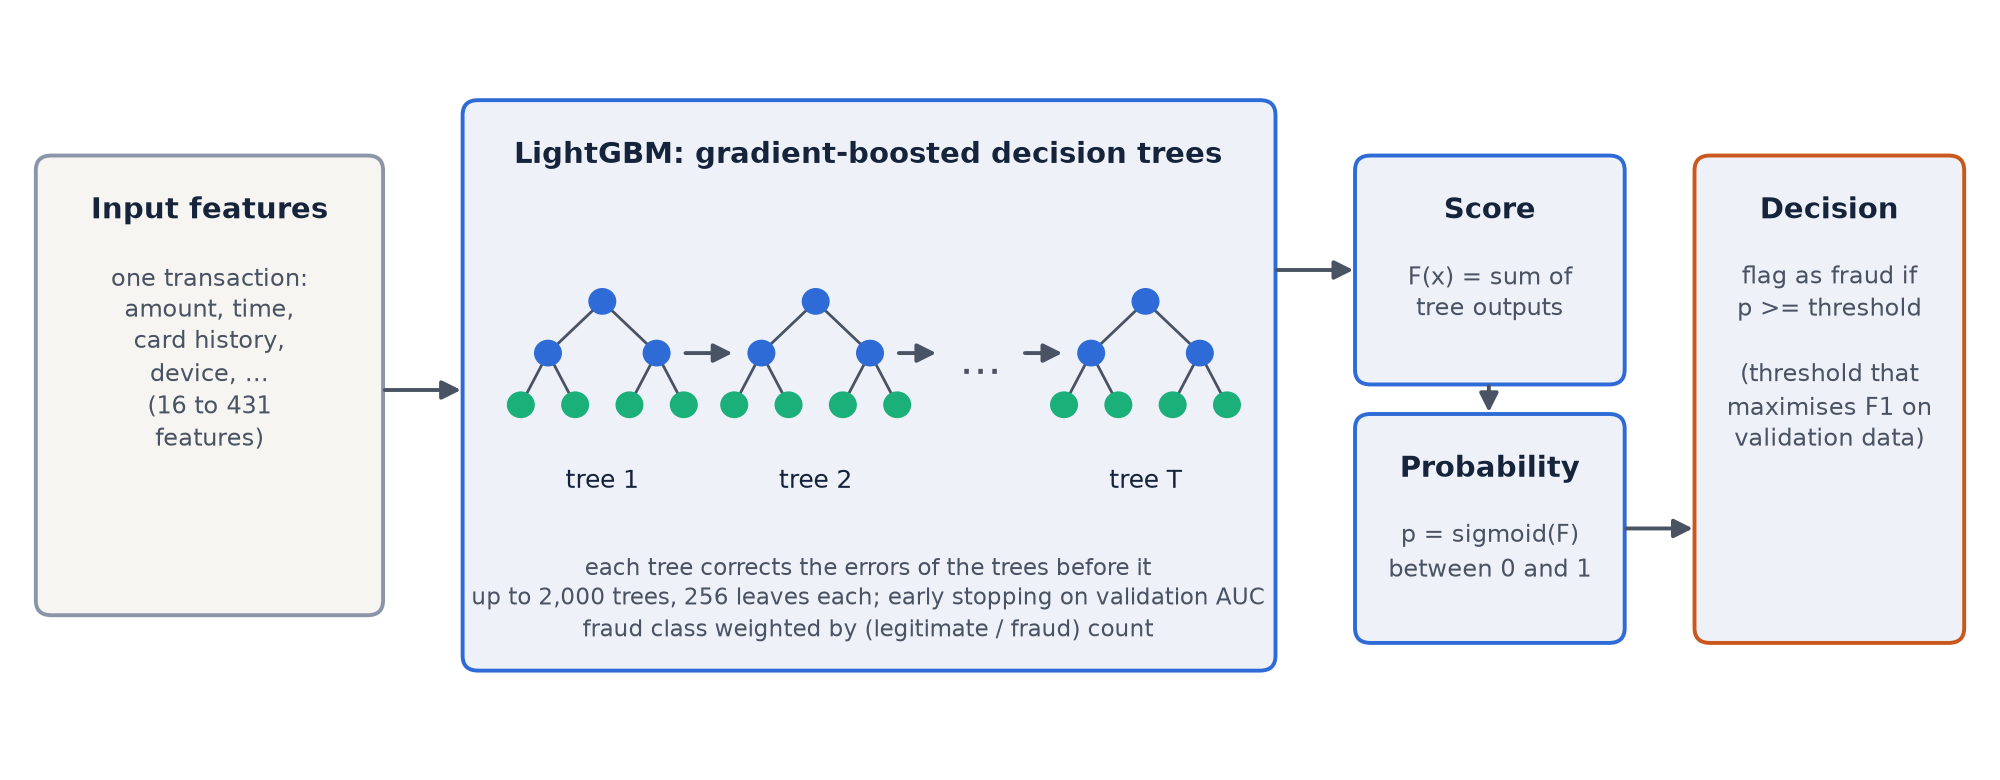
\includegraphics[width=\textwidth]{figures/model_architecture.png}
  \caption{Architecture of the fraud detection model: a transaction's features pass through a sequence of boosted decision trees, whose summed output becomes a fraud probability and, with the validation threshold, a decision}
  \label{fig:modelarch}
\end{figure}

{\footnotesize
\begin{longtable}{>{\raggedright\arraybackslash}p{0.32\textwidth}>{\raggedright\arraybackslash}p{0.19\textwidth}>{\raggedright\arraybackslash}p{0.43\textwidth}}
\caption{LightGBM settings used for every model in the study}\label{tab:hyper}\\
\toprule
\textbf{Setting} & \textbf{Value} & \textbf{Purpose} \\
\midrule
\endfirsthead
\toprule
\textbf{Setting} & \textbf{Value} & \textbf{Purpose} \\
\midrule
\endhead
Objective & binary & Fraud probability for each transaction \\ \midrule
Learning rate & 0.05 & Step size of each boosting round \\ \midrule
Number of leaves & 256 & Capacity of each tree \\ \midrule
Minimum samples per leaf & 100 & Prevents leaves fitted to a few transactions \\ \midrule
Row subsampling & 0.8, every round & Randomness and regularisation \\ \midrule
Feature subsampling & 0.5 per tree & Randomness and regularisation \\ \midrule
L2 regularisation & 1.0 & Shrinks leaf values \\ \midrule
Class weight of fraud & legitimate / fraud count in the training data & Compensates for class imbalance \\ \midrule
Boosting rounds & up to 2,000, early stopping after 100 without improvement & Stops on the validation part of the training window \\ \midrule
Validation part & most recent 15\% of the training window & Early stopping, threshold choice and reference PR-AUC \\ \bottomrule
\end{longtable}
}

Every training run uses a time-ordered validation split: the most recent 15\% of the training window is held out for early stopping, for choosing the decision threshold, and for recording the model's reference PR-AUC. The decision threshold is the one that maximises the F1-score on this validation part. It is used for the F1-score, precision and recall reported alongside PR-AUC and for the fraud flags returned by the scoring service; PR-AUC itself does not depend on a threshold. Alessi and Fugini manage the threshold dynamically during operation to balance precision and recall \cite{alessi2026}; in this design each model keeps the threshold chosen at training time, and a new threshold arrives with every retrained model.

For the static baseline in RQ1, the first 50\% of each dataset is used for training, the next 10\% for validation, and the remaining 40\% is divided into ten consecutive time bins, so that performance can be followed over the months after deployment.

\subsection{Framework Architecture}\label{sec:arch}

The framework turns the experimental findings into a working MLOps system. Its components are shown in Figure \ref{fig:architecture} and its settings in Table \ref{tab:framework}. It runs the loop of Figure \ref{fig:loop} every seven days: monitor, decide, retrain, check, and serve. Like the closed-loop MLOps framework of Reda et al. for phishing detection \cite{reda2025}, it connects monitoring, retraining and deployment in one automated loop; unlike it, its decisions are designed for weeks of label delay rather than near-immediate feedback, so retraining follows a schedule instead of being driven by drift events.

\begin{figure}[htbp]
  \centering
  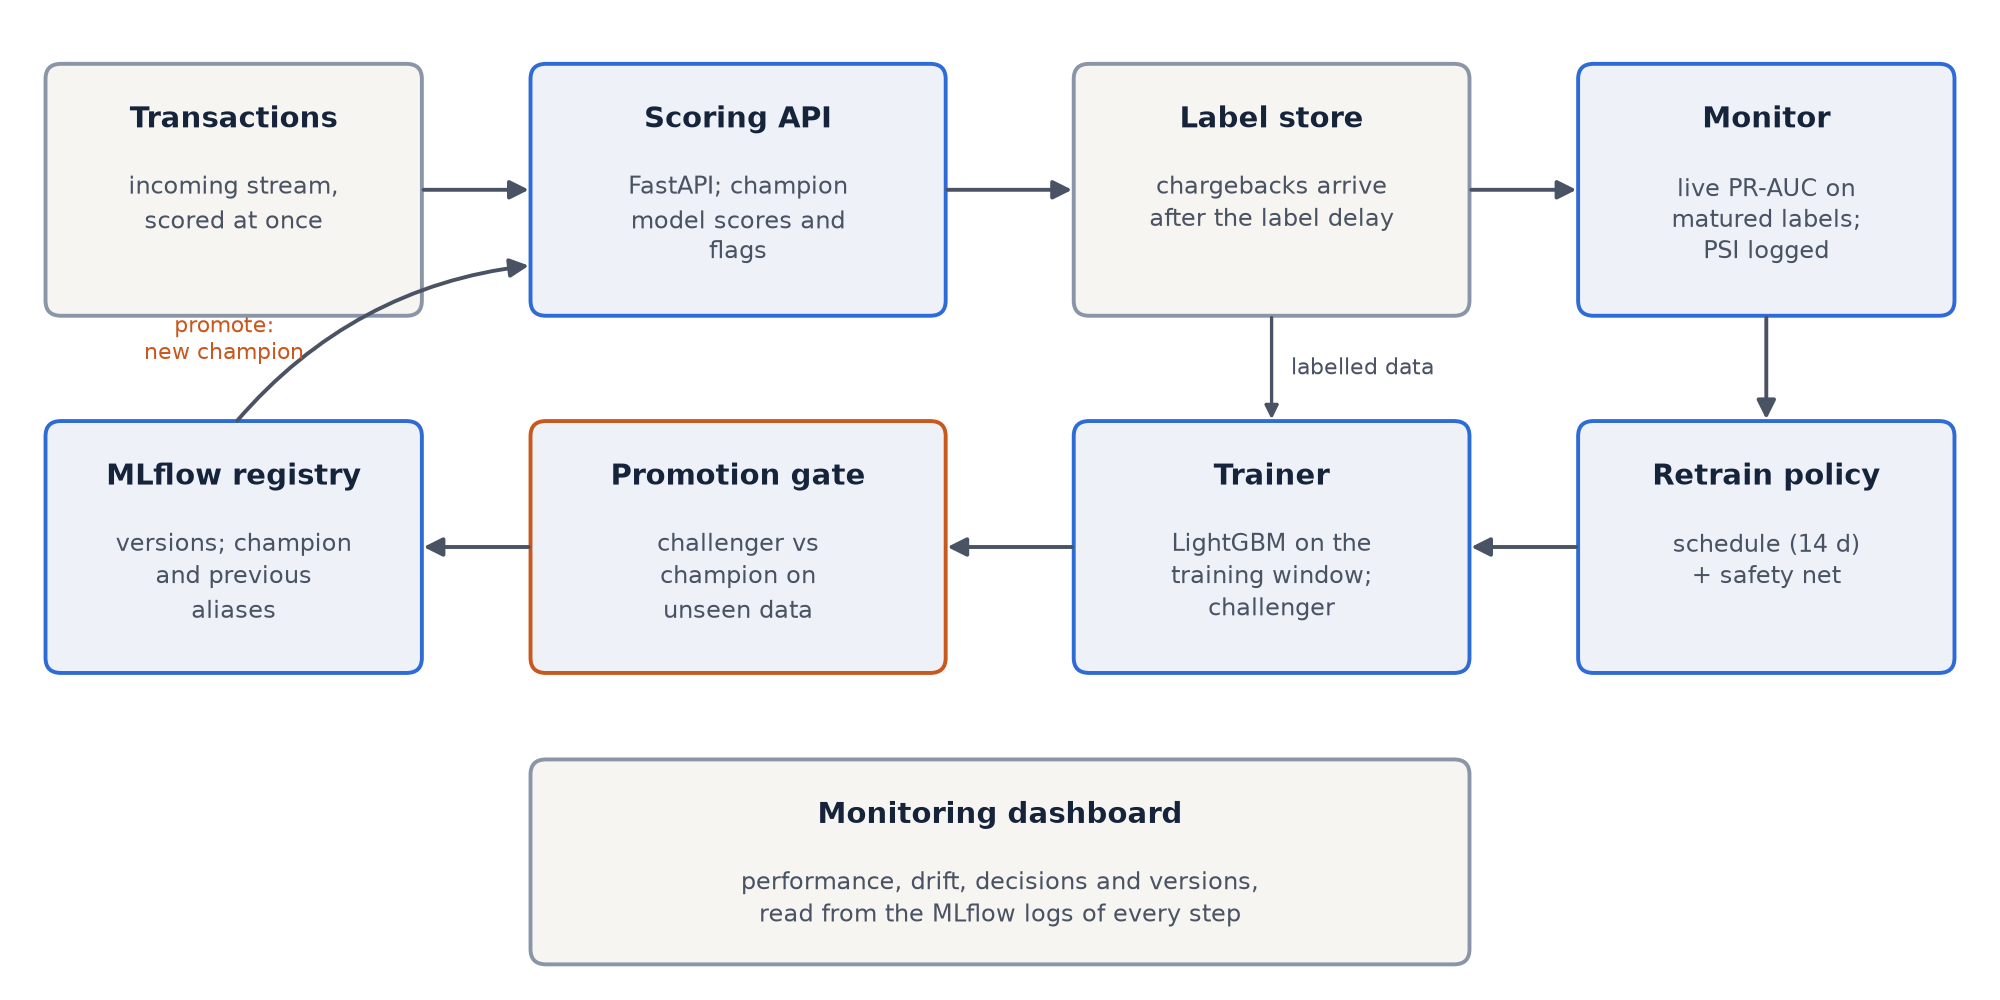
\includegraphics[width=\textwidth]{figures/architecture.png}
  \caption{Components of the proposed framework and the flow of data between them}
  \label{fig:architecture}
\end{figure}

\subsection{Monitoring on Delayed Labels}\label{sec:monitor}

The monitor measures the live model's PR-AUC on the labels that matured during the last 14 days, restricted to transactions the model was not trained on. It also computes the PSI of the model's scores and of its ten most important numeric features against a sample of 50,000 rows of its training window, and logs both to MLflow. In line with the experimental results, the PSI is logged for diagnosis only and never triggers retraining on its own. Two forms of monitoring are deliberately left outside the current design: tracking drift separately for each source of data, as DriftGuard-TriAudit does for the numbers, text and layout of financial statements \cite{hassan2026}, and tracking the stability of model explanations, which John showed can become unstable and unfair as populations drift \cite{john2025}. Both are natural extensions once the framework is used with several data sources or with explanations shown to investigators.

\subsection{Retraining Policy and Safety Net}\label{sec:safety}

The primary policy is a fixed schedule: a new model is trained every 14 days on the last 60 days of labelled data. The schedule is complemented by a \textit{safety net} that retrains early, at most once every seven days, when performance collapses between scheduled retrains:

\begin{equation}
  \mathrm{AP}_{\mathrm{live}} < (1 - \tau)\,\max\big(\mathrm{AP}_{\mathrm{val}},\ \mathrm{median}_{4}(\mathrm{AP}_{\mathrm{live}})\big)\quad\text{or}\quad \mathrm{AP}_{\mathrm{live}} < \lambda\,\pi
  \label{eq:safety}
\end{equation}

with $\tau$ = 0.30, $\lambda$ = 3 and $\pi$ the fraud rate among the matured labels. The first condition compares live PR-AUC with the better of the model's own validation PR-AUC and the median of the last four live measurements. Using recent live history as well as the validation score matters: a model trained on corrupted data can report a poor validation score, which would otherwise lower the bar it is measured against. The second condition is a no-skill check, since a model without skill has a PR-AUC close to the fraud rate.

\subsection{Training and Automatic Window Selection}\label{sec:window}

The trainer fits a LightGBM model with the settings of Table \ref{tab:hyper} on the policy's training window, which ends one label delay before the present. The window length can be set to zero for an expanding window. Each new model is registered in MLflow as a \textit{challenger}, together with its training window, validation PR-AUC and threshold.

\textbf{Automatic window selection.} The experiments showed that the best training window depends on the dataset: the last 60 days on IEEE-CIS, but all labelled history on Sparkov and BAF. A fixed window chosen on one dataset can be wrong for another. The framework can therefore select the window itself. At every retrain it trains one challenger \textit{m\textsubscript{w}} per candidate window \textit{w}, here the last 60 days and all labelled history, and scores all of them on the same evaluation rows \textit{E}: the most recent labelled transactions that none of the candidates was trained on and the champion was not trained on either. It keeps

\begin{equation}
  w^{*} = \arg\max_{w \in \mathcal{W}} \mathrm{AP}_{E}(m_w), \qquad \mathcal{W} = \{\text{60 days},\ \text{all history}\}
  \label{eq:select}
\end{equation}

and only this challenger goes on to the promotion gate; the others are registered as not selected. The choice uses only data that would be available at the time, so it needs no knowledge of which window suits the dataset. Because the candidates are trained on identical data except for their start date, the extra cost is one additional training run per retrain.

\subsection{Promotion Gate}\label{sec:gate}

A challenger replaces the live model (the \textit{champion}) only if it passes the promotion gate, following the champion-challenger pattern of MLOps practice \cite{pulicharla2019,kodakandla2024}. The gate compares both models on the challenger's validation data, restricted to transactions that the champion was not trained on, so that neither model is judged on data it has seen. The challenger is promoted if

\begin{equation}
  \mathrm{AP}(\text{challenger}) \ge \mathrm{AP}(\text{champion}) - \delta
  \label{eq:gate}
\end{equation}

with $\delta$ = 0.01. Both models are re-scored through the production feature path rather than with scores stored at training time. This detail is essential: a model trained on wrongly scaled features looks good on its own, equally wrong, validation data, but fails on the inputs it will actually receive in production. If the comparison data contains fewer than 30 frauds, the comparison is not reliable and the challenger is promoted by default.

\subsection{Framework Configuration}\label{sec:config}

{\footnotesize
\begin{longtable}{>{\raggedright\arraybackslash}p{0.32\textwidth}>{\raggedright\arraybackslash}p{0.15\textwidth}>{\raggedright\arraybackslash}p{0.47\textwidth}}
\caption{Settings of the framework (configs/default.toml)}\label{tab:framework}\\
\toprule
\textbf{Setting} & \textbf{Value} & \textbf{Meaning} \\
\midrule
\endfirsthead
\toprule
\textbf{Setting} & \textbf{Value} & \textbf{Meaning} \\
\midrule
\endhead
Loop interval & 7 days & How often the framework monitors, decides and serves \\ \midrule
Label delay d & 30 days & Labels usable this long after the transaction \\ \midrule
Retraining schedule & 14 days & Primary policy \\ \midrule
Training window & 60 days & Sliding window of labelled data (0 = expanding) \\ \midrule
Candidate windows & 60 days, all & With automatic selection: one challenger per window, the best one is gated \\ \midrule
Monitoring window & 14 days & Matured labels used for live PR-AUC \\ \midrule
Minimum frauds & 30 & Fewer frauds: live PR-AUC is not computed \\ \midrule
Safety-net tolerance $\tau$ & 0.30 & Relative drop that triggers an early retrain \\ \midrule
History for the reference & 4 & Recent live measurements in the median \\ \midrule
No-skill factor $\lambda$ & 3 & Live PR-AUC below 3 x fraud rate triggers \\ \midrule
Minimum gap between retrains & 7 days & Prevents repeated early retrains \\ \midrule
Gate tolerance $\delta$ & 0.01 & Largest PR-AUC loss a challenger may show \\ \midrule
Gate minimum frauds & 30 & Fewer frauds: the challenger is promoted by default \\ \midrule
Drift features tracked & 10 & Most important numeric features (PSI logged) \\ \bottomrule
\end{longtable}
}

\section{Data Collection}\label{sec:collection}

The study uses three public fraud datasets, summarised in Table \ref{tab:sources}. Public data with reliable timestamps is essential for the research questions, because drift and label delay can only be studied when transactions can be replayed in the order in which they happened. Commonly used fraud datasets that cover only a few days \cite{dang2021,mienye2023} were therefore not suitable.

{\footnotesize
\begin{longtable}{>{\raggedright\arraybackslash}p{0.15\textwidth}>{\raggedright\arraybackslash}p{0.32\textwidth}>{\raggedright\arraybackslash}p{0.23\textwidth}>{\raggedright\arraybackslash}p{0.24\textwidth}}
\caption{Sources of the datasets}\label{tab:sources}\\
\toprule
\textbf{Dataset} & \textbf{Source} & \textbf{Files used} & \textbf{Records in the source} \\
\midrule
\endfirsthead
\toprule
\textbf{Dataset} & \textbf{Source} & \textbf{Files used} & \textbf{Records in the source} \\
\midrule
\endhead
IEEE-CIS & Kaggle competition IEEE-CIS Fraud Detection (IEEE Computational Intelligence Society and Vesta Corporation) & train\_transaction.csv, train\_identity.csv & 590,540 transactions \\ \midrule
Sparkov & Kaggle dataset Credit Card Transactions Fraud Detection (generated with the Sparkov simulator) & fraudTrain.csv, fraudTest.csv & 1,852,394 transactions \\ \midrule
BAF & Kaggle dataset Bank Account Fraud Dataset Suite (NeurIPS 2022) & Base.csv (of six variants) & 1,000,000 applications \\ \bottomrule
\end{longtable}
}

All three datasets were downloaded from Kaggle. IEEE-CIS is distributed as a competition dataset, which requires accepting the competition rules; its test files have no labels and were not used. Sparkov is distributed as two files that split one continuous period, and both were combined. BAF is distributed as a base dataset and five variants with controlled biases; the base dataset was used. The raw data is not redistributed with the code: the repository contains the scripts that prepare it, so that every result can be regenerated from the original sources.

Two practical choices made the data collection reproducible. First, every dataset is converted by a preparation script into the same table layout, so all experiments run unchanged on any of them. Second, the long experiments on the two larger replication datasets were run as Kaggle notebooks, next to the data, with the code taken directly from the public repository.

\section{Dataset Overview}\label{sec:data}

This section describes each dataset, the target variable, the cleaning and feature engineering applied to it, and the resulting preprocessed data.

\subsection{IEEE-CIS Fraud Detection}\label{sec:ieeecis}

IEEE-CIS is the main dataset. It was released by the IEEE Computational Intelligence Society and Vesta Corporation and contains 590,540 real e-commerce transactions over 182 days, of which 3.5\% are fraudulent. It has been used in recent studies of drift and fraud detection \cite{menezes2025,uddin2026}. The transaction and identity tables are joined on the transaction identifier, giving 431 features, most of them anonymised by the provider. Only the time column (seconds from a reference point), the identifier and the label are excluded. Text columns are treated as categorical features, which LightGBM handles natively, and missing values are kept as missing rather than imputed. More than half of the columns are missing for over 50\% of transactions.

\subsection{Sparkov Credit Card Transactions}\label{sec:sparkovds}

Sparkov is the first replication dataset. It contains card transactions for about 1,000 customers produced by the Sparkov transaction simulator between January 2019 and December 2020. After inspection we cut the data at 21 December 2020, because the simulator produces almost no fraud after that date (17 frauds and then none, while the volume doubles), which would make the last weeks meaningless for evaluation. The remaining 1,801,969 transactions cover 720 days with a fraud rate of 0.53\%. Names, street addresses, card numbers and transaction numbers are removed. We derive the transaction hour and weekday, the customer's age, and the distance between customer and merchant, and five per-card behaviour features: the time since the card's previous transaction, its number and total amount of transactions in the previous 24 hours, its number of transactions in the previous 30 days, and the amount relative to the card's running average. Each of these is computed only from the card's \textit{earlier} transactions, so no information from the future leaks into a feature. A lifetime transaction count was deliberately not used: it only grows over time and would drift by construction.

\subsection{Bank Account Fraud (BAF)}\label{sec:bafds}

BAF is the second replication dataset. It is a privacy-preserving synthetic dataset of one million bank account applications over eight months, generated from real data and designed to contain realistic drift between months. We use the Base variant. Values that the providers document as missing (negative values in six columns) are converted to missing values, a constant column is dropped, and the month itself is not used as a feature, so that the model cannot memorise the period. BAF records only the month of each application, so each record is given a random time within its month with a fixed seed. Drift therefore appears between months, while the weeks within a month are exchangeable. This is a limitation of the dataset, and the BAF results are interpreted accordingly.

\subsection{Target Variable and Class Imbalance}\label{sec:target}

The target is a binary label that marks a transaction, or an application in the case of BAF, as fraudulent (1) or legitimate (0). It is called isFraud in IEEE-CIS, is\_fraud in Sparkov and fraud\_bool in BAF, and is renamed isFraud in all three. Fraud is rare in every dataset: there are 27.6 legitimate transactions per fraud in IEEE-CIS, 186.1 in Sparkov and 89.7 in BAF. For this reason accuracy is not used as a measure (a model that never predicts fraud would be 96.5\% to 99.5\% accurate), and PR-AUC is the main measure (Section \ref{sec:measures}). The imbalance is handled by weighting the fraud class in training; no oversampling such as SMOTE is used, because resampling can make results look better than they are \cite{dang2021}.

\subsection{Data Cleaning and Feature Engineering}\label{sec:cleaning}

The preprocessing pipeline is shown in Figure \ref{fig:preproc}. In IEEE-CIS, the transaction and identity tables are joined on the transaction identifier, numeric columns are stored in the smallest suitable type to reduce memory, and the 31 text columns are converted to categorical features. Missing values are kept as missing, because LightGBM handles them natively and because missingness itself can carry information: 214 of the 434 columns are missing for more than half of the transactions.

In Sparkov, names, street addresses, card numbers and transaction numbers are removed, and the data is cut at 21 December 2020, after which the simulator produces almost no fraud; this keeps 1,801,969 of 1,852,394 transactions. Time-of-day, weekday, age and the distance between customer and merchant are derived, and five per-card behaviour features are computed only from each card's earlier transactions, so that no information leaks from the future. In BAF, values documented as missing (negative values in six columns) are converted to missing, a constant column is dropped, and the month is not used as a feature.

\begin{figure}[htbp]
  \centering
  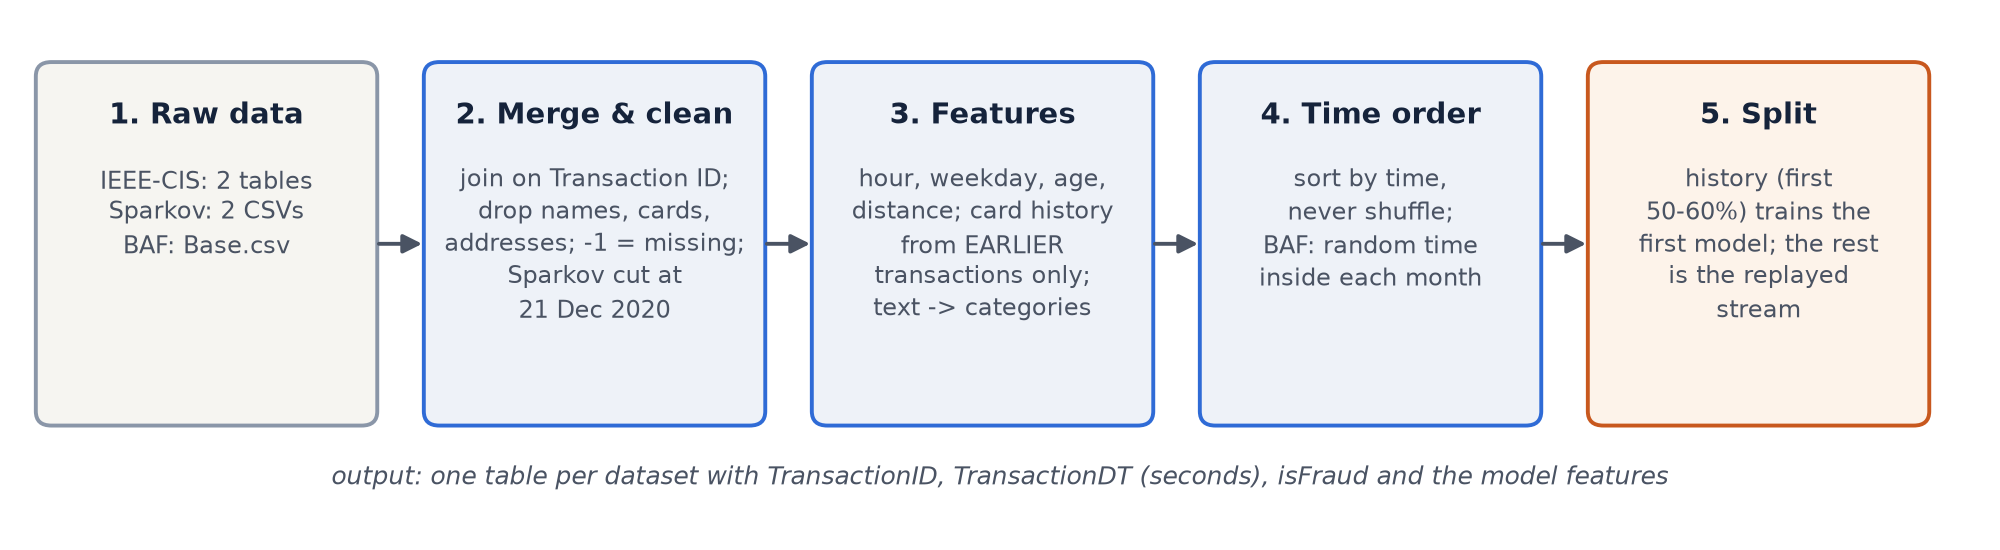
\includegraphics[width=\textwidth]{figures/preprocessing.png}
  \caption{Preprocessing pipeline from the raw files of each dataset to the common time-ordered table}
  \label{fig:preproc}
\end{figure}

\subsection{Time Ordering and History-Stream Split}\label{sec:split}

All three datasets are sorted by time and never shuffled. Each is split at a fixed fraction of its rows into a \textit{history}, used to train the first model, and a \textit{stream}, which is replayed as if it were arriving live (Figure \ref{fig:protocol}). The stream starts at 60\% of the rows for IEEE-CIS (day 101), and at 50\% for Sparkov and BAF, whose longer histories allow a full year or four months of training data before deployment.

\begin{figure}[htbp]
  \centering
  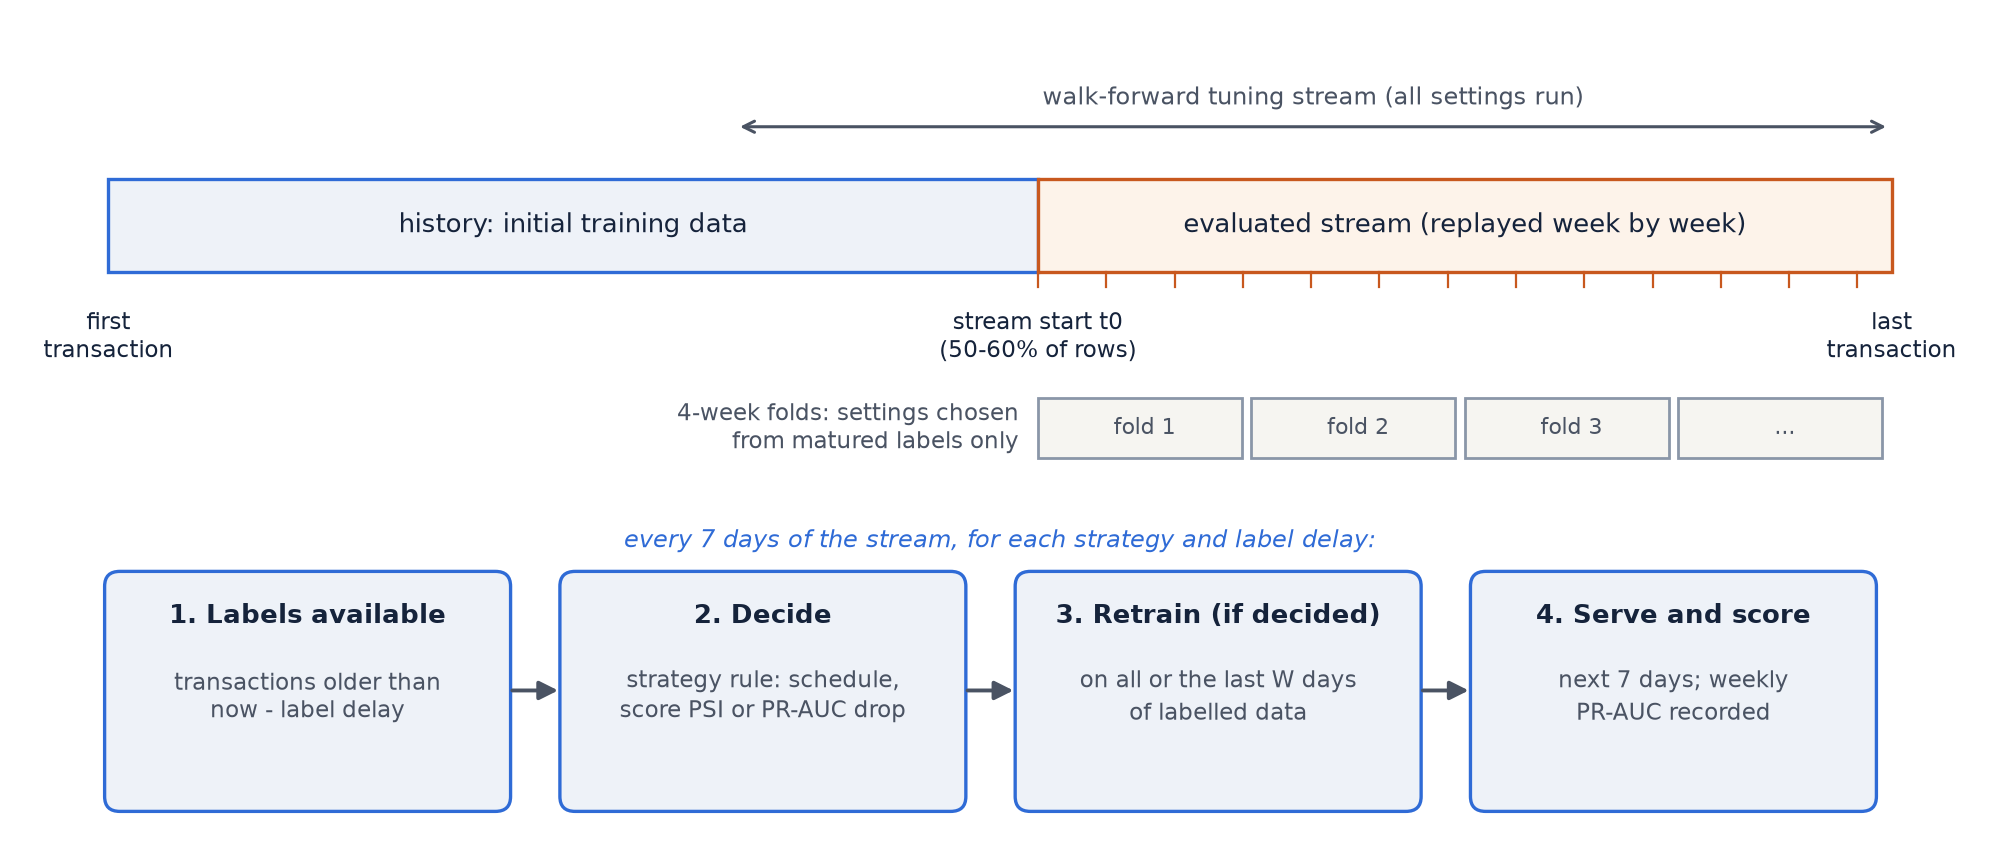
\includegraphics[width=\textwidth]{figures/protocol.png}
  \caption{Evaluation protocol: each dataset is split in time into a history and a stream that is replayed week by week; settings are tuned walk-forward in 4-week folds}
  \label{fig:protocol}
\end{figure}

\subsection{Summary of Preprocessed Data}\label{sec:summarydata}

Table \ref{tab:preprocessed} summarises the data after preprocessing, and Table \ref{tab:datasets} compares the three datasets. Every prepared dataset is a single table with a transaction identifier, a time column in seconds, the isFraud label and the model features, sorted by time.

{\footnotesize
\begin{longtable}{>{\raggedright\arraybackslash}p{0.32\textwidth}>{\raggedright\arraybackslash}p{0.21\textwidth}>{\raggedright\arraybackslash}p{0.21\textwidth}>{\raggedright\arraybackslash}p{0.21\textwidth}}
\caption{Summary of the preprocessed data}\label{tab:preprocessed}\\
\toprule
\textbf{} & \textbf{IEEE-CIS} & \textbf{Sparkov} & \textbf{BAF} \\
\midrule
\endfirsthead
\toprule
\textbf{} & \textbf{IEEE-CIS} & \textbf{Sparkov} & \textbf{BAF} \\
\midrule
\endhead
Records after preprocessing & 590,540 & 1,801,969 & 1,000,000 \\ \midrule
Frauds (rate) & 20,663 (3.50\%) & 9,634 (0.53\%) & 11,029 (1.10\%) \\ \midrule
Legitimate per fraud & 27.6 & 186.1 & 89.7 \\ \midrule
Features (of which categorical) & 431 (31) & 16 (5) & 29 (5) \\ \midrule
History: training the first model & 354,324 (60\%) & 900,984 (50\%) & 500,000 (50\%) \\ \midrule
Stream: replayed week by week & 236,216 (12 weeks) & 900,985 (52 weeks) & 500,000 (19 weeks) \\ \bottomrule
\end{longtable}
}

{\footnotesize
\begin{longtable}{>{\raggedright\arraybackslash}p{0.16\textwidth}>{\raggedright\arraybackslash}p{0.26\textwidth}>{\raggedright\arraybackslash}p{0.26\textwidth}>{\raggedright\arraybackslash}p{0.25\textwidth}}
\caption{Datasets used in this study (after preparation)}\label{tab:datasets}\\
\toprule
\textbf{} & \textbf{IEEE-CIS} & \textbf{Sparkov} & \textbf{BAF (Base)} \\
\midrule
\endfirsthead
\toprule
\textbf{} & \textbf{IEEE-CIS} & \textbf{Sparkov} & \textbf{BAF (Base)} \\
\midrule
\endhead
Domain & Real e-commerce card transactions (Vesta) & Simulated card transactions (Sparkov generator) & Bank account opening applications (privacy-preserving synthetic data) \\ \midrule
Records & 590,540 & 1,801,969 & 1,000,000 \\ \midrule
Time span & 182 days & 720 days (to 21 Dec 2020) & 8 months \\ \midrule
Fraud rate & 3.50\% & 0.53\% & 1.10\% \\ \midrule
Features used & 431 (transaction and identity tables, mostly anonymised) & 16 (amount, time, location, customer and card-history features) & 29 (applicant, request, device and velocity features) \\ \midrule
Time resolution & Seconds from a reference point & Exact timestamp & Month only (time within the month assigned at random) \\ \midrule
Stream starts at & 60\% of rows (day 101) & 50\% of rows (about 1 Jan 2020) & 50\% of rows (month 4) \\ \midrule
Role & Main dataset & Replication & Second replication \\ \bottomrule
\end{longtable}
}

\section{Project Management Plan}\label{sec:plan}

The project was organised in three stages that match the thesis deliverables, as shown in Figure \ref{fig:plan}. The first stage covered the literature review, the research questions and the preparation of IEEE-CIS. The second stage covered the experiments, their statistical validation and the design of the framework. The third stage covered the framework's evaluation, the replication on two further datasets, automatic window selection and the changes requested in supervisor feedback.

\begin{figure}[htbp]
  \centering
  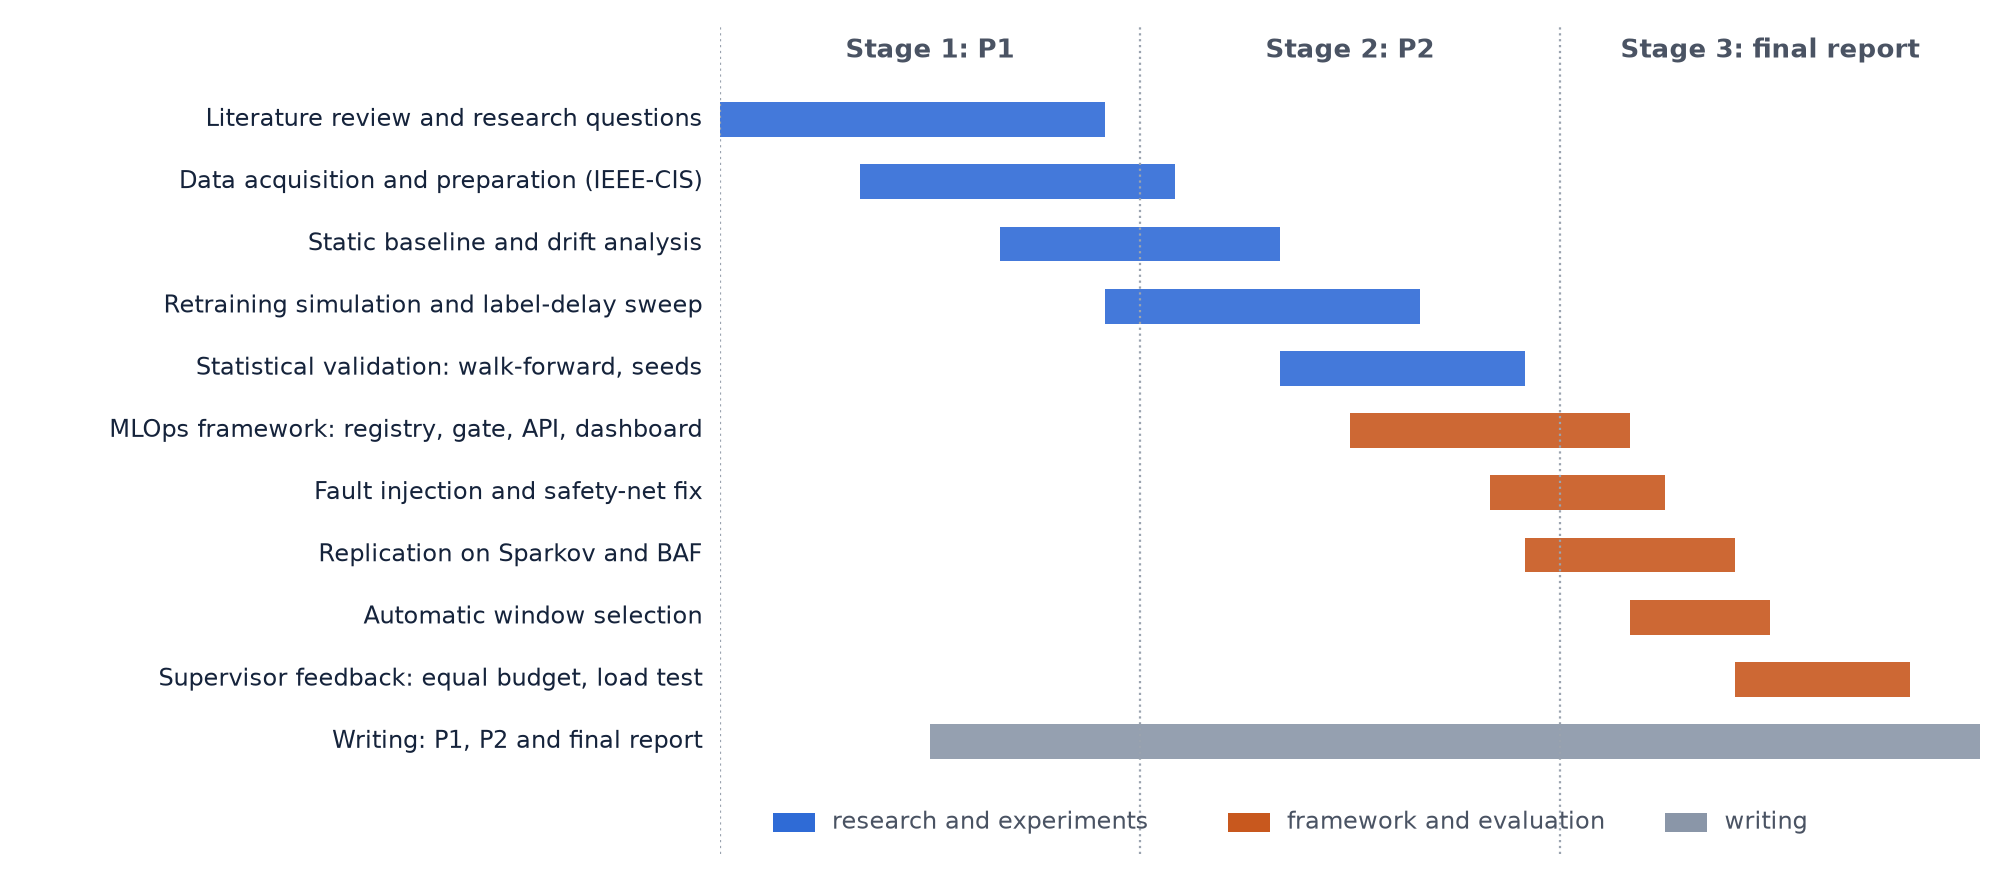
\includegraphics[width=\textwidth]{figures/project_plan.png}
  \caption{Project management plan over the three thesis stages}
  \label{fig:plan}
\end{figure}

Work proceeded in short iterations: each experiment was planned, run, reviewed and, when its result raised a new question, followed by a further experiment. Several design decisions came out of this cycle. The walk-forward tuning was added when fixed tuning periods proved too short to rank the drift triggers; the promotion gate was changed to re-score models on production features after a fault test exposed a weakness; and automatic window selection was added when the replication showed that the best window depends on the dataset. Supervisor feedback was incorporated in the same way, for example the equal-budget comparison in Section \ref{sec:budget}.

All code and configuration were kept under version control in a Git repository hosted on GitHub, with an automated test suite run before each change. Because single experiments ran for several hours and power cuts were frequent, the long experiments save their results after every completed step and resume where they stopped; the longest runs were moved to Kaggle notebooks.

\section{Implementation of Selected Design}\label{sec:impl}

The selected design was implemented as a Python package with a back end that runs the continuous learning loop, a front end for monitoring, and a model registry that connects them. Table \ref{tab:modules} lists the modules.

\subsection{Back End}\label{sec:backend}

{\footnotesize
\begin{longtable}{>{\raggedright\arraybackslash}p{0.21\textwidth}>{\raggedright\arraybackslash}p{0.73\textwidth}}
\caption{Modules of the framework (Python package fraud\_mlops)}\label{tab:modules}\\
\toprule
\textbf{Module} & \textbf{Responsibility} \\
\midrule
\endfirsthead
\toprule
\textbf{Module} & \textbf{Responsibility} \\
\midrule
\endhead
config & Typed configuration loaded from one TOML file per dataset \\ \midrule
data & Loading, caching and time-window access to the transaction table \\ \midrule
training & LightGBM training on a window with a time-ordered validation split \\ \midrule
model & Scoring of raw input, including missing columns and text categories \\ \midrule
monitoring & Live PR-AUC on matured labels; PSI of scores and features \\ \midrule
policy & Retraining policy, safety net, candidate windows and promotion gate \\ \midrule
registry & MLflow runs and model registry with champion and previous aliases \\ \midrule
pipeline & The replay loop: monitor, decide, retrain, gate and serve \\ \midrule
faults & Fault injection for testing the safeguards \\ \midrule
serving & FastAPI scoring service for the champion model \\ \midrule
dashboard & Self-contained HTML monitoring dashboard \\ \midrule
cli & Command line: replay, champion, dashboard and serve \\ \bottomrule
\end{longtable}
}

The study is implemented in Python with LightGBM, pandas, NumPy and scikit-learn for the experiments, MLflow with an SQLite backend for tracking and the model registry, and FastAPI for the scoring service. The framework is organised as a Python package with separate modules for configuration, data access, training, monitoring, the retraining policy, the promotion gate, the registry, fault injection, serving and the dashboard, and is configured with one TOML file per dataset. Twenty-four automated tests on small synthetic data check the components and the full loop.

The back end is driven from the command line. \textit{replay} runs the loop over a dataset as if it were live, \textit{champion} reports the model in service, \textit{dashboard} builds the monitoring dashboard and \textit{serve} starts the scoring service. Every training run is logged to MLflow with its parameters, metrics and training window, and every model is registered as a new version.

\subsection{Front End}\label{sec:frontend}

The front end is a monitoring dashboard, generated as a single HTML page from the MLflow logs of a replay, that can be opened in any browser without a server. It shows the summary figures of the run, the weekly performance of the served model together with what the loop could measure on delayed labels and the safety-net line (Figure \ref{fig:dashtop}), the drift measures, every retraining decision with its reason, and the history of model versions with the champion and the version kept for rollback (Figure \ref{fig:dashlog}).

\begin{figure}[htbp]
  \centering
  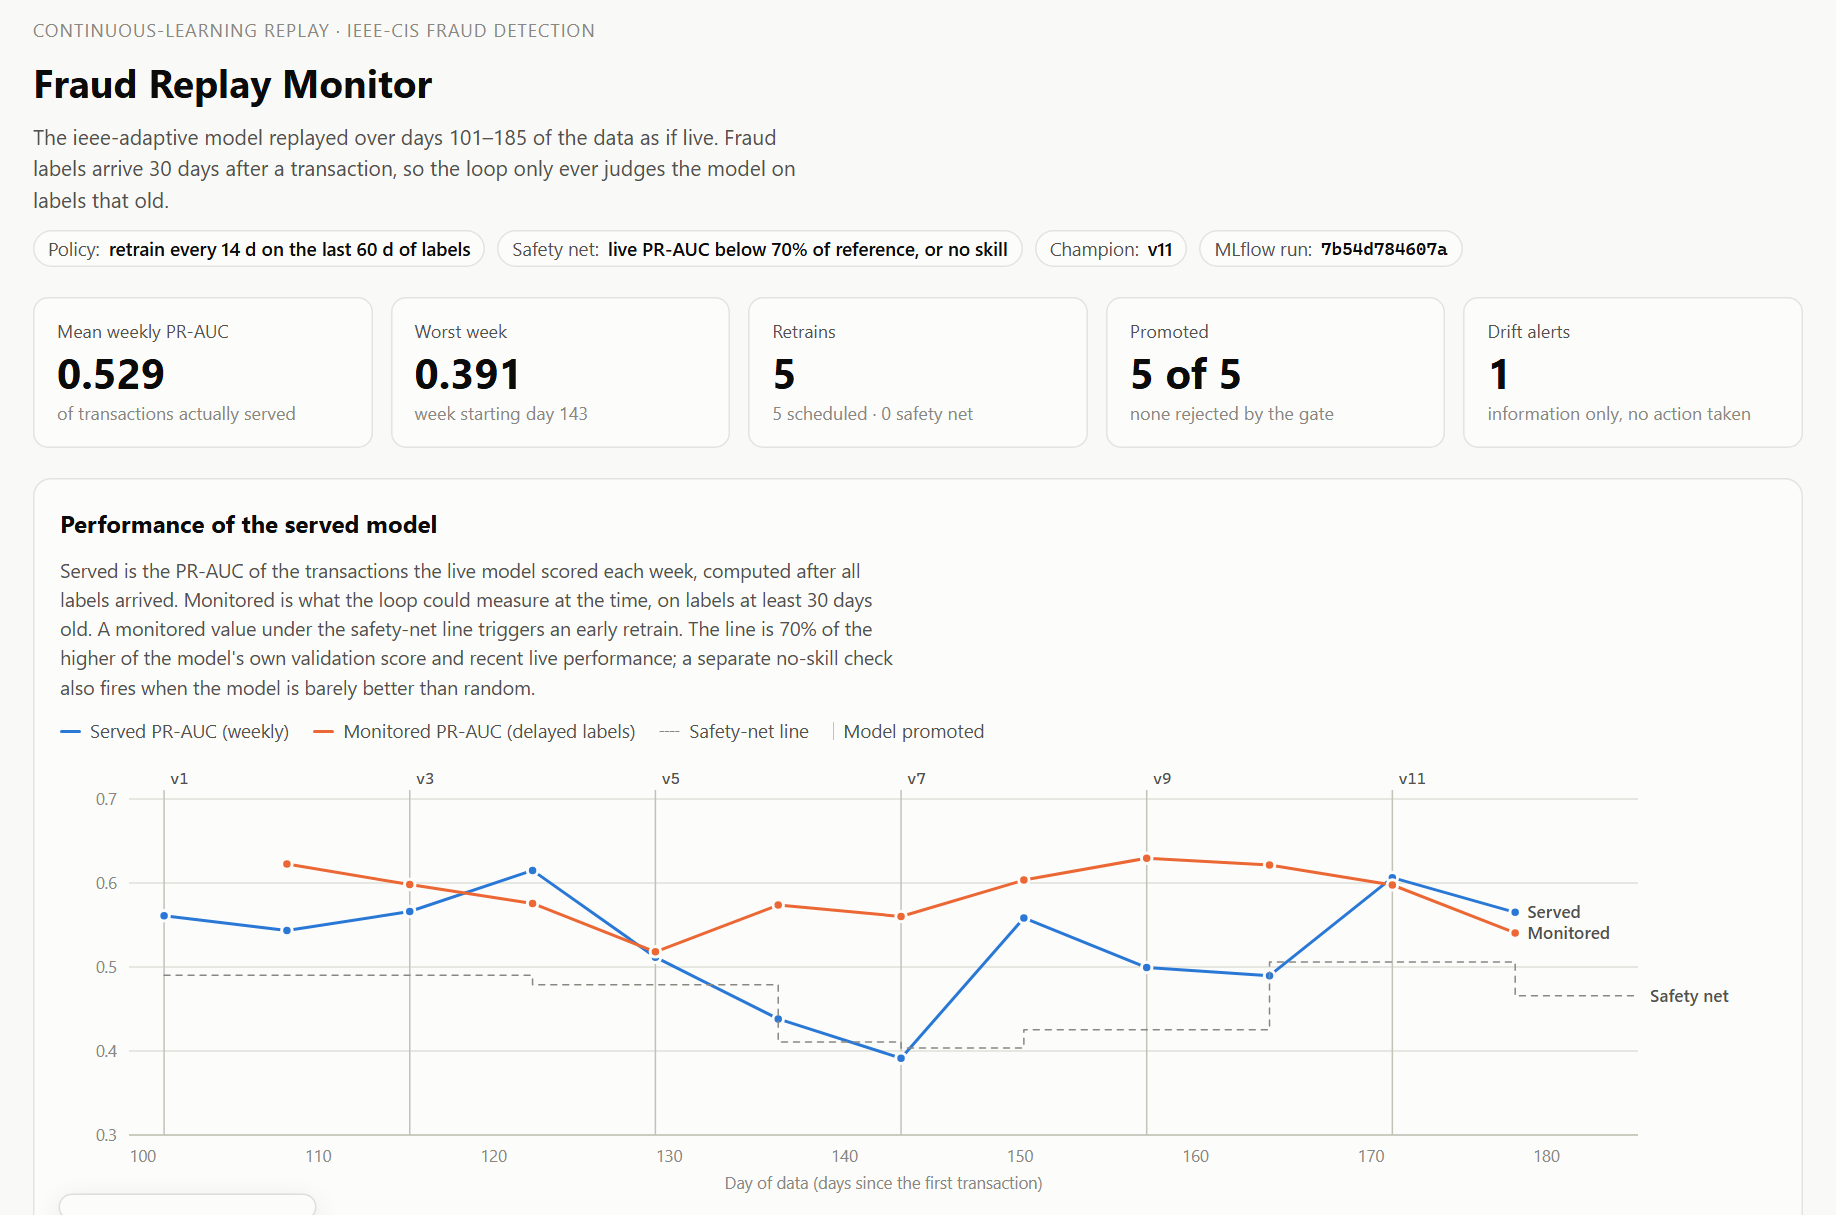
\includegraphics[width=\textwidth]{figures/dashboard_top.png}
  \caption{Front end: the monitoring dashboard after a replay of IEEE-CIS (summary figures and the performance of the served model)}
  \label{fig:dashtop}
\end{figure}

\begin{figure}[htbp]
  \centering
  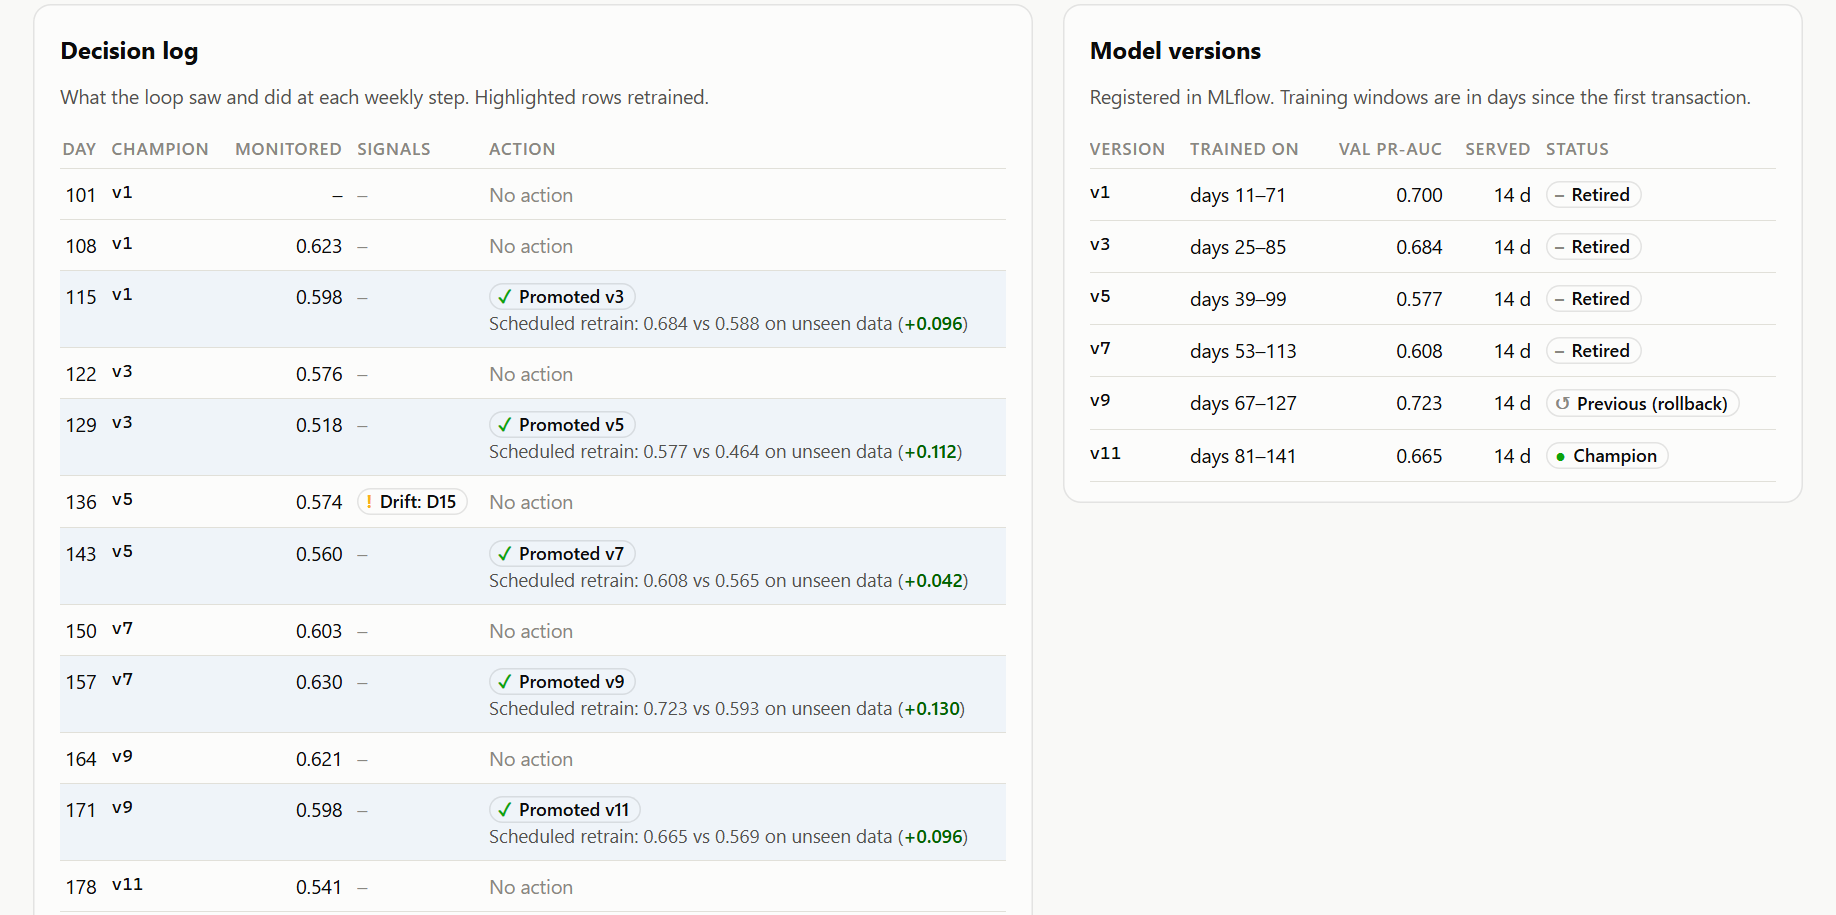
\includegraphics[width=\textwidth]{figures/dashboard_log.png}
  \caption{Front end: decision log and model versions on the monitoring dashboard}
  \label{fig:dashlog}
\end{figure}

\subsection{Frontend-Backend Integration}\label{sec:integration}

MLflow stores every model version with its parameters, metrics and training window. The model in service carries the alias \textit{champion} and its predecessor the alias \textit{previous}, so a rollback is a single alias change. A FastAPI service loads the champion and offers three endpoints: \textit{/health} reports the version being served, \textit{/predict} returns a fraud probability and flag for each submitted transaction, and \textit{/reload} switches to a newly promoted champion without restarting. A monitoring dashboard, generated from the MLflow logs, shows weekly performance, drift, every retraining decision with its reason, and the history of model versions.

The MLflow model registry is the contract between the parts: the back end writes model versions and moves the \textit{champion} alias when the promotion gate accepts a challenger, the scoring service loads whatever carries that alias and reloads it on request, and the dashboard reads the same registry and run logs. No component needs to know how the others work, so the scoring service always serves the model the gate last approved.
